\newpage 
%\section{Methodology}¨
%\chapter{Methodology}
%\label{sec:methodology}

\chapter{Review of state of the art anomaly detectors}
%\section{Evaluation of RX, LRX and ACAD }
%\label{sec:MATLAB_methodology}
\label{chapter:review_anomaly_detectors}
To evaluate the performance of the ADs considered in this task, models of the algorithms described in section \ref{sec:anomaly_detectors_theory} were developed in MATLAB, and tested on both hyperspectral image data from the Cuprite site \cite{Cuprite_data} taken by NASA's AVIRIS hyperspectral imager and synthetic images created by the author. 
\\

The MATLAB hyperspectral toolbox \cite{MATLAB_hyperspectral_toolbox} was used for image preprocessing, visualization and for having a good starting point for developing further functionality. The toolbox included an implementation of the RX algorithm. A fork of the toolbox was made, available at \cite{MATLAB_hyperspectral_toolbox_fork}, to be able to do MATLAB implementations of LRX, ALRX and ACAD in order to evaluate the performance of the ADs. The most important scripts and functions from the forked toolbox are also located in appendix \ref{appendice:MATLAB_hyperspectral}.
\section{Experiments on Synthetic images testing}
To make an objective analysis  of the considered ADs performance, synthetic hyperspectral images with known anomalies were created. The images contained anomalies of various sizes, to test the ADs ability to detect variably sized anomalies. A similar test is also done in \cite{global_and_local_rx}. Figure 7(a) in \cite{global_and_local_rx} shows that the RX algorithm was not able to detect anomalies in the third and four column (anomalous pixels made up of >50\% abundance of the anomaly signature). The LRX exhibit slightly better anomaly detection accuracy in this test.
\\

The purpose of the synthetic images used in this thesis was to get objective metrics of the performance of the evaluated ADs. Two different metrics are important in order to evaluate the performance of the ADs; $false\_anomalies$ and $\%correctly\_predicted\_anomalies$. These metrics are defined in equation \ref{eq:false_anomalies_metric} and \ref{eq:correctly_predicted_anomalies_metric}. The value $true\_anomalies$ is taken from the reference anomaly map created during the creation of the synthetic images. These values are important as they provide an objective metric to evaluate the performance of the ADs, something that can not be done with real hyperspectral image data, unless one posesses a reference anomaly map to the real image data, which the author has not been able to find.  

% If this is bigger than >0, else 0
\begin{equation}
    false\_anomalies = predicted\_anomalies - true\_anomalies
    \label{eq:false_anomalies_metric}
\end{equation}


\begin{equation}
    \%correctly\_predicted\_anomalies= \frac{predicted\_anomalies-false\_anomalies}{true\_anomalies}
    \label{eq:correctly_predicted_anomalies_metric}
\end{equation}

Synthetic images with different image size and anomaly sizes were created to evaluate the performance of the ADs. To be able to compare to the tests done on images with a size of 200x200 as described in chapter 5.5.1 in \cite{hsueh_master_thesis} by Hsueh, these tests were mimicked. The synthetic image can be seen in figure \ref{fig:hsueh_image}. In addition, synthetic images with size of 30 x 30 pixels were created with an anomalous panel of size 2x2 inserted into the center of the images. This image scene is labelled as $Sim30\_30AVIRIS$. The anomalous pixels are pure pixels with a spectral signature of Buddingtonite. These images has a background consisting of $33\%$ Alunite, $33\%$ Kalonite and $33\%$ Pyrope, extracted from the Cuprite image scene \cite{ground_truth_cuprite}. Such a generated synthetic image can be seen in Figure \ref{fig:synthetic_30_30}.


\begin{figure}[H]
\begin{minipage}[]{.5\linewidth}
\centering
\subfloat[ 200 x 200 synthetic image.]{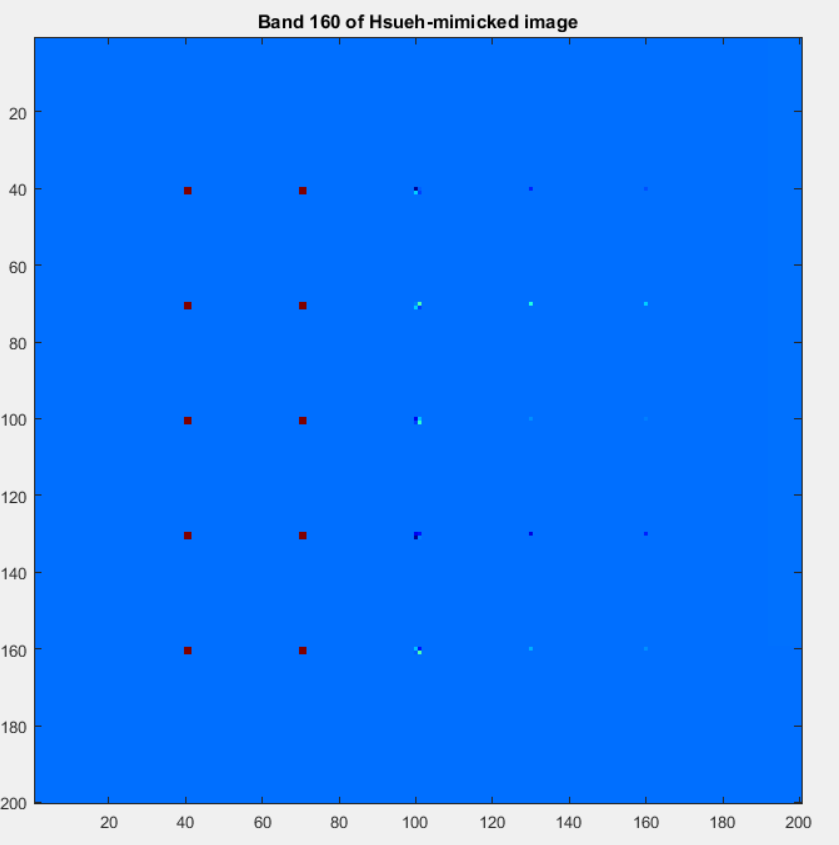
\includegraphics[scale=.5]{images/AD_testing/synthetic_images/band_160_hsueh_picture_without_gaussian_noise.PNG}}
  %\caption{Lena 256 x 256 uncompressed. Used for testing of MATLAB SPIHT script.}
  %\label{fig:lena_unc}
\end{minipage}%
\begin{minipage}[]{.5\linewidth}
\centering
  \subfloat[Synthetic image with added Gaussian white noise with a SNR of 20:1.]{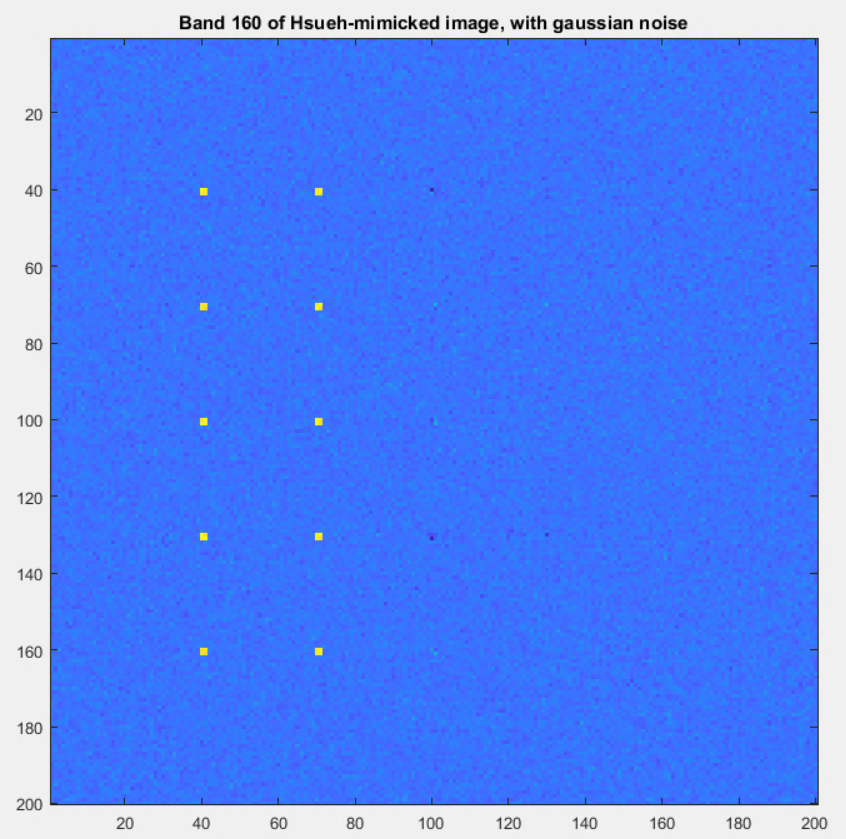
\includegraphics[scale=.5]{images/AD_testing/synthetic_images/band_160_hsueh_picture_with_gaussian_noise.PNG}}
  %\caption{Lena 256 x 256 reconstructed after being compressed having 0.1 bpp, using the MATLAB SPIHT script. See appendix. }
  %\label{fig:lena_comp}
\end{minipage}


\caption{First class of synthetic images: 200 x 200 synthetic image with 25 inserted anomaly panels as describe by Hsueh in \cite{hsueh_master_thesis}. Displaying spectral band 160. }
\label{fig:hsueh_image}
\end{figure}

\begin{figure}[H]
\centering
   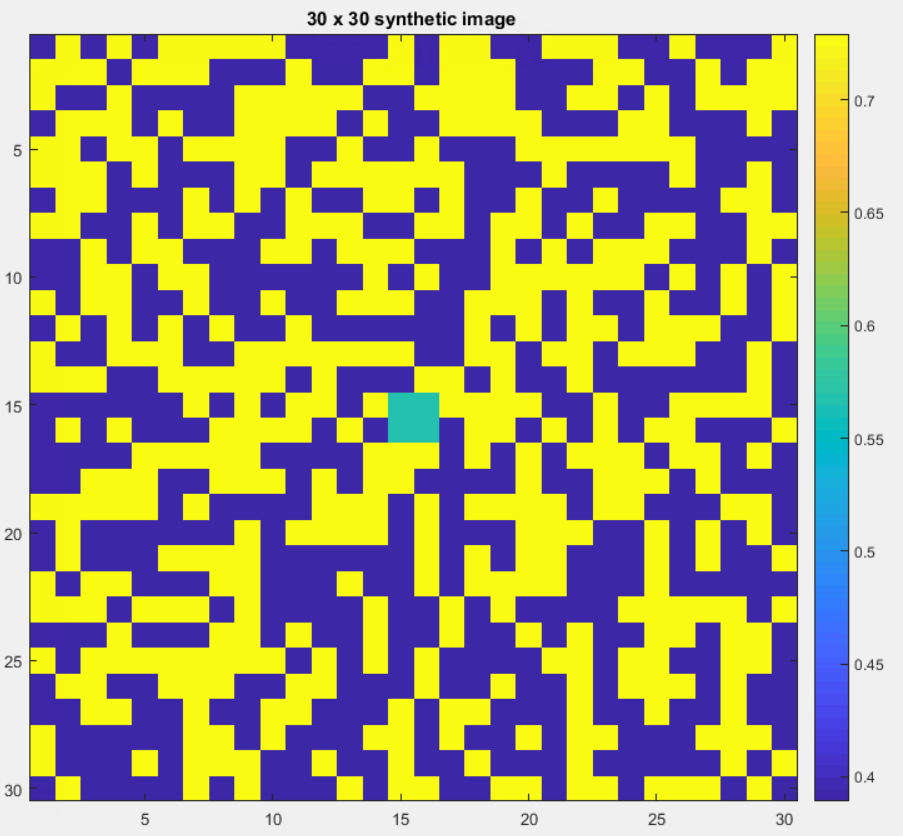
\includegraphics[scale=0.4]{images/AD_testing/synthetic_images/30_30_anomaly_image.PNG}
  \caption{Second class of synthetic images: Synthetic 30x30 image with an inserted 2x2 anomalous panel inserted into the center. Displaying spectral band 160. } 
  \label{fig:synthetic_30_30}
\end{figure}


\\
A third class of synthetic images with a size of $100$ x $614$ pixels was also created. These images had a background consisting of $33\%$ Alunite, $33\%$ Kalonite and $33\%$ Pyrope. The anamalous pixels are pure pixels with a spectral signature of Buddingtonite, extracted from the Cuprite image scene \cite{ground_truth_cuprite}. Six different sized anomalous-target kernels were made, with a size of $1x1$, $2x2$, $5x5$, $10x10$, $15x15$, $20x20$ and $25x25$ pixels.




\begin{table}[H]
\centering
\caption{Properties of the third class of synthetic images used in experiments. Row and column locations are location of the center pixel in the kernel of size $k x k$.}
\label{tab:synthetic_images}
\begin{tabular}{l|l|l|l}
\textbf{Scene} & \textbf{Row} & \textbf{Column} & \textbf{Anomaly size {[}pixels x pixels{]}} \\
SimAviris01    & 35           & 50              & 1x1                                         \\
SimAviris01    & 70           & 50              & 1x1                                         \\
SimAviris01    & 35           & 100             & 2x2                                         \\
SimAviris01    & 70           & 100             & 2x2                                         \\
SimAviris01    & 35           & 150             & 5x5                                         \\
SimAviris01    & 70           & 150             & 5x5                                         \\
SimAviris01    & 35           & 250             & 10x10                                       \\
SimAviris01    & 70           & 250             & 10x10                                       \\
SimAviris01   & 35           & 350             & 15x15                                       \\
SimAviris01    & 70           & 350             & 15x15                                       \\
SimAviris01    & 35           & 450             & 20x20                                       \\
SimAviris01    & 70           & 450             & 20x20                                       \\
SimAviris01    & 35           & 550             & 25x25                                       \\
SimAviris01    & 70           & 550             & 25x25                                      
\end{tabular}
\end{table}



\begin{figure}[H]
\hbox{\hspace*{-0}                                              
   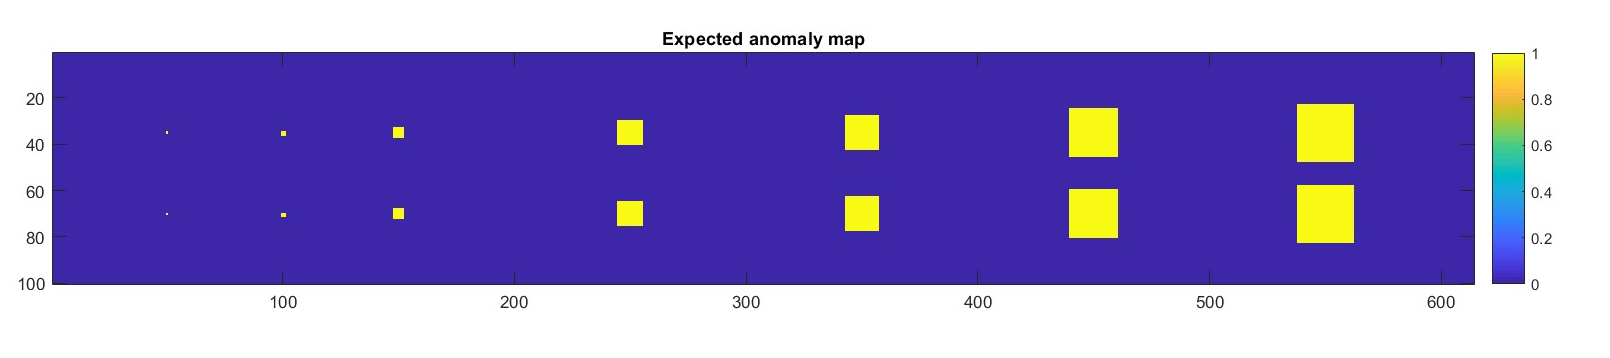
\includegraphics[scale=0.4]{images/AD_testing/synthetic_images/expected_anomaly_map.png}}
  \caption{Expected anomaly map for the third class of synthetic images created.} 
  \label{fig:anomaly_map_615_100}
\end{figure}

\subsection{RX}
Since the RX AD does not build an anomaly map, the author defines anomalous pixels as pixels having a score of $\geqslant$ 75\% of the max value outputted from the RX AD. This is done in order to be able to set the objective metrics $false\_anomalies$ and $\%correctly\_predicted\_anomalies$ for the RX detector in order to compare it to the other evaluated ADs. 

\subsubsection{Hsueh-mimicked image}

\begin{figure}[H]
\begin{minipage}[]{.5\linewidth}
\centering
\subfloat[ RX AD result for synthetic image shown in \ref{fig:hsueh_image}. ]{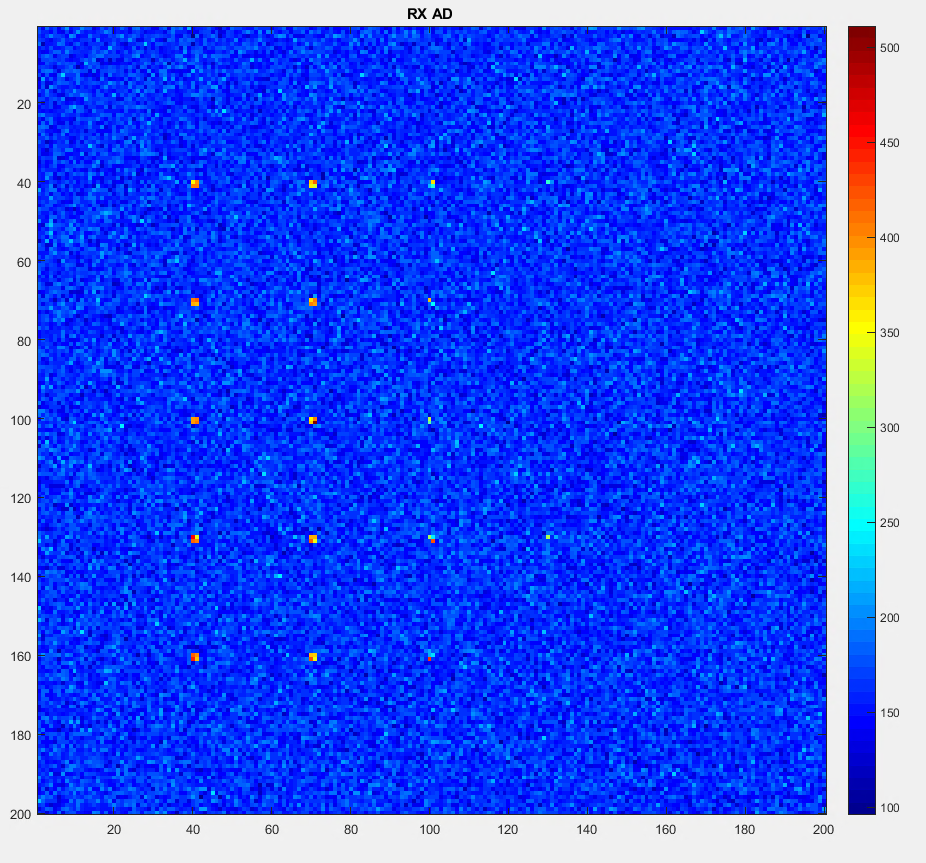
\includegraphics[scale=.35]{images/AD_testing/synthetic_images/rx_ad_hshueh.PNG}}
  %\caption{Lena 256 x 256 uncompressed. Used for testing of MATLAB SPIHT script.}
  %\label{fig:lena_unc}
\end{minipage}%
\begin{minipage}[]{.5\linewidth}
\centering
  \subfloat[Generated anomaly map for RX, setting threshold value for what is considered an anomaly as $\geqslant$ 75\% of the max value of the RX AD.]{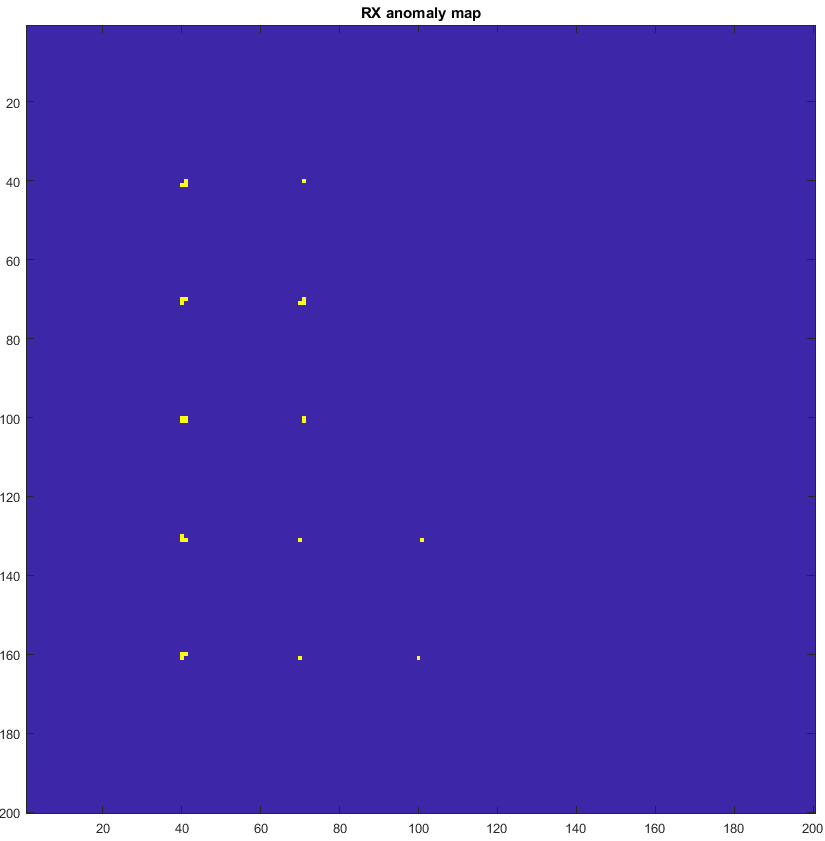
\includegraphics[scale=.3]{images/AD_testing/synthetic_images/rx_hsueh_anomaly_map.PNG}}
  %\caption{Lena 256 x 256 reconstructed after being compressed having 0.1 bpp, using the MATLAB SPIHT script. See appendix. }
  %\label{fig:lena_comp}
\end{minipage}


\caption{RX AD test on synthetic image based on Hsueh's description. The map in (b) was created to provide a way of computing $false\_anomalies$ and $ \%correctly\_predicted\_anomalies$.  }
\label{fig:hsueh_image_RX_test}
\end{figure}

The value of $false\_anomalies$ = 0, and  $\%correctly\_predicted\_anomalies$ = $0.3714$ for this test.

\subsubsection{$Sim30\_30AVIRIS$ scene }
\begin{figure}[H]
\centering
   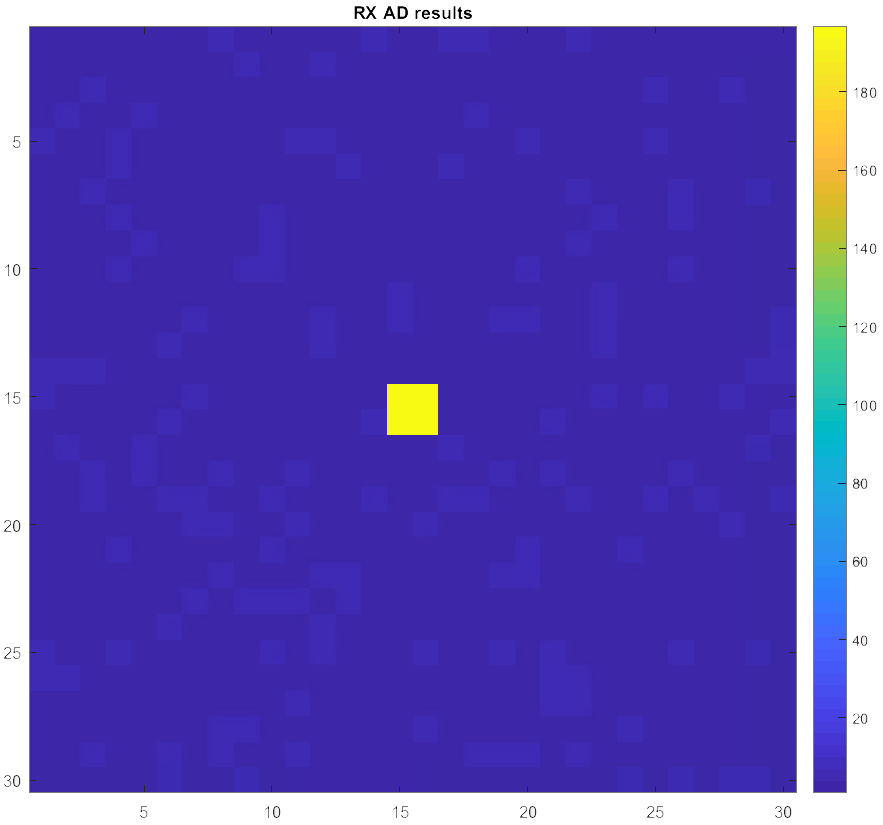
\includegraphics[scale=0.4]{images/AD_testing/synthetic_images/rx_ad_30_30.png}
  \caption{ RX AD results for the $Sim30\_30AVIRIS$ scene.} 
  \label{fig:rx_sim_aviris_30_30}
\end{figure}

The value of $false\_anomalies$ = 0, and  $\%correctly\_predicted\_anomalies$ = $1$ for this test.


\subsubsection{$Sim\_Aviris01$ scene }
\begin{figure}[H]
\hbox{\hspace*{-1cm}                                              
   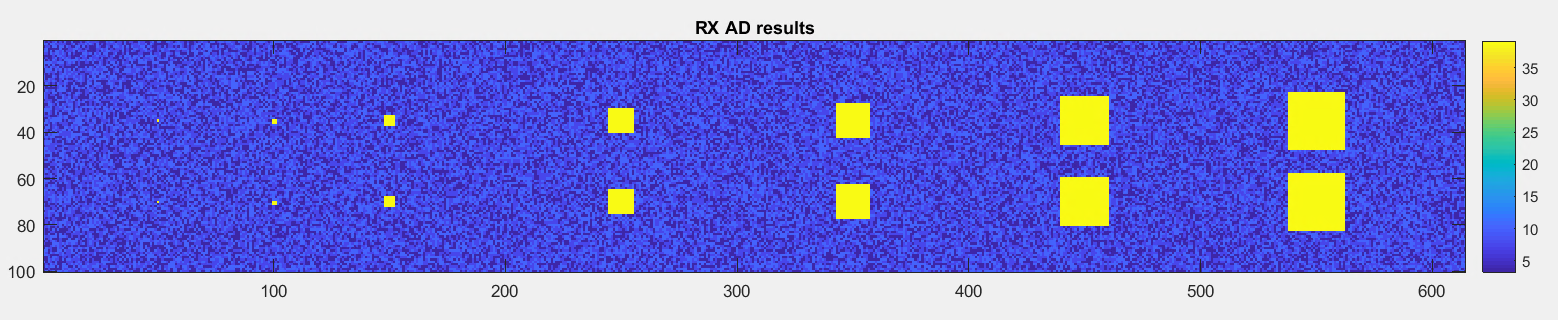
\includegraphics[scale=0.4]{images/AD_testing/synthetic_images/rx_ad_614_100.png}}
  \caption{ RX AD results for the $Sim\_Aviris01$ scene.} 
  \label{fig:rx_sim_aviris_01}
\end{figure}

The value of $false\_anomalies$ = 0, and  $\%correctly\_predicted\_anomalies$ = $1$ for this test.

\subsection{LRX}

\subsection{ALRX}

\subsection{ACAD}


\section{Testing on data from real images}
To evaluate the performance of the ADs considered in this task they were tested on hyperspectral image data from the Cuprite mining area captured by the AVIRIS hyperspectral camera.
 Band 220 from Cuprite scene 02 can be seen in figure \ref{fig:cuprite_scene_band_220}. The real image data does not provide a means for calculating objective metrics such as $false\_anomalies$ and $\%correctly\_predicted\_anomalies$, but gives an impression of the considered ADs performance when applied to real image data.

\begin{figure}[H]

\hbox{\hspace*{-1cm}                                                           

   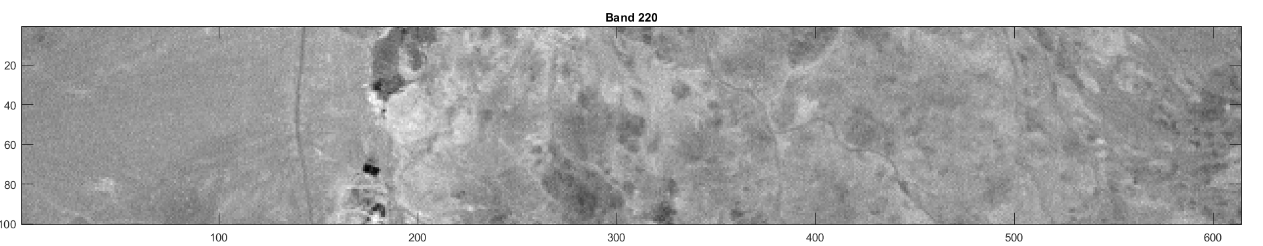
\includegraphics[scale=0.65]{images/AD_testing/original_band_220_22_1.png}}
  \caption{Spectral band 220 from the hyperspectral data set of the Cuprite site\cite{Cuprite_data}. } 
  \label{fig:cuprite_scene_band_220}
\end{figure}


\subsection{RX}
As described in section \ref{sec:RX_theory}, the RX algorithm computes the covariance on the global set of pixel vectors to indicate the probability of a pixel being an anomalous pixel. 

\begin{figure}[H]

\hbox{\hspace*{-2cm}                                                           

   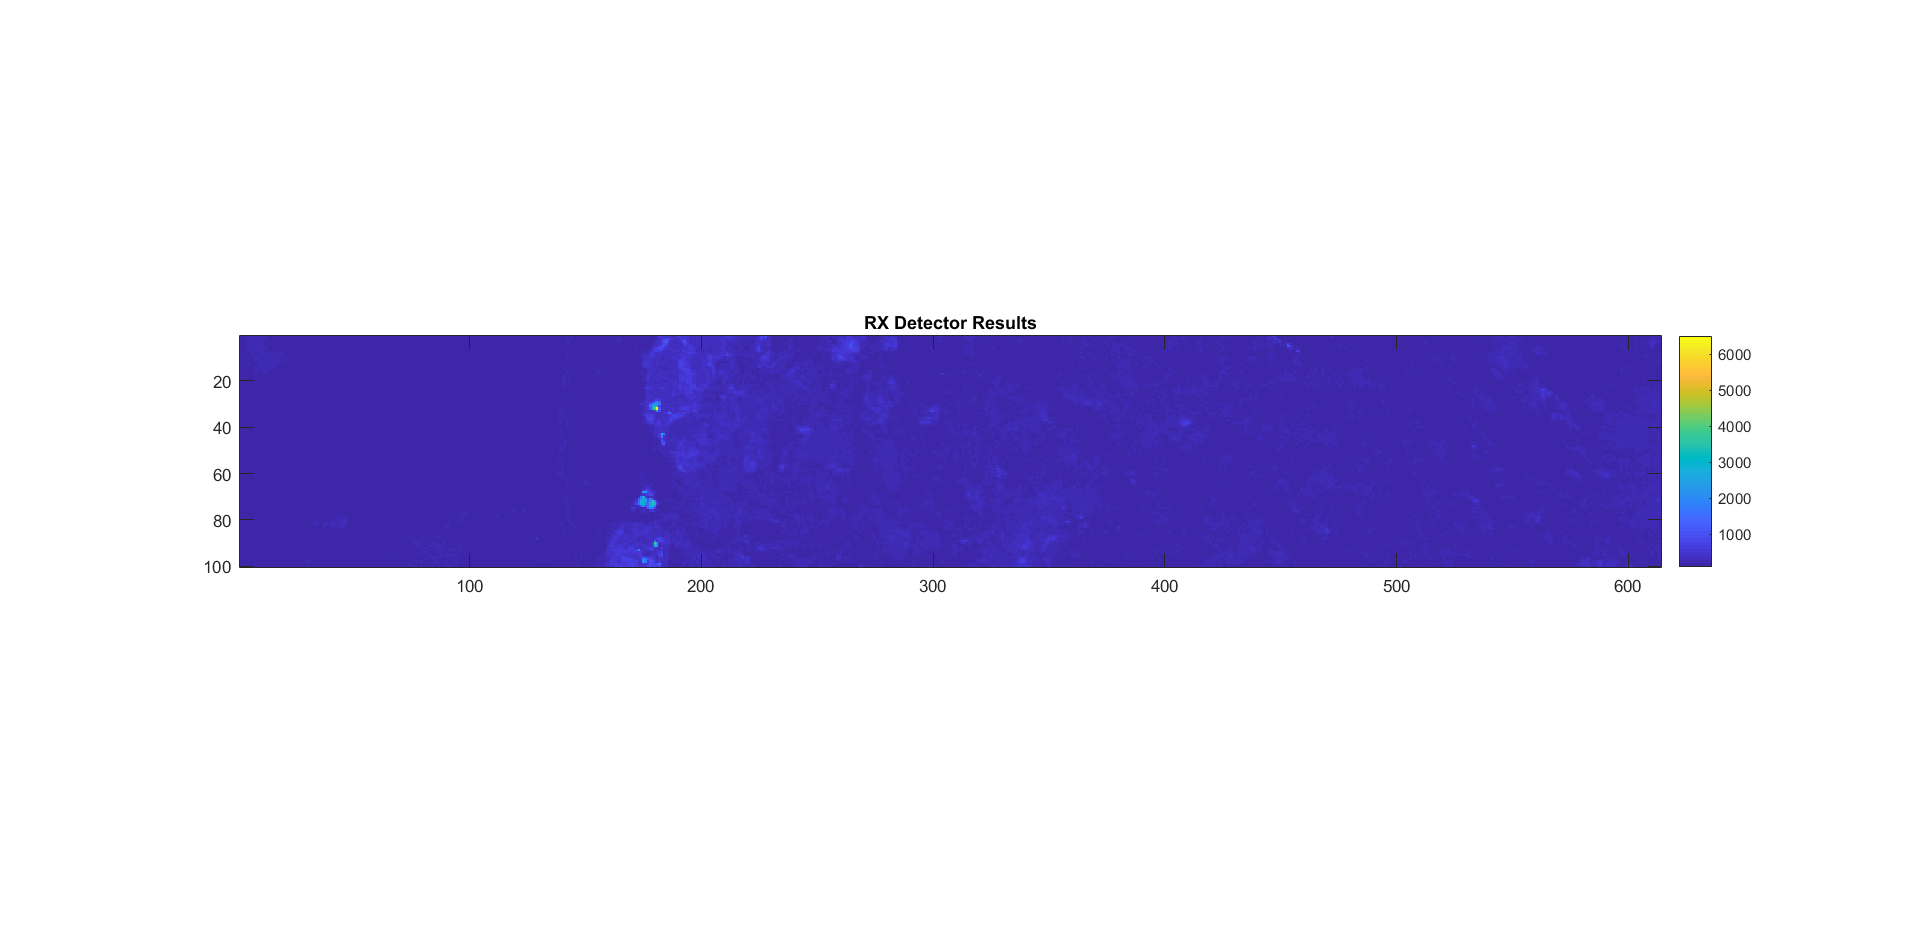
\includegraphics[scale=0.4]{images/AD_testing/GRX_22_1.png}}
  \caption{Result from RX AD on Cuprite image data. Higher score indicates higher probability of the pixel being anomalous. } 
  \label{fig:cuprite_scene_band_220}
\end{figure}



\subsection{LRX}
LRX computes the correlation matrix on a pixel vector block of size $K$ in order to detect anomalous pixel vectors, as described in section \ref{sec:LRX_theory}. 

\begin{figure}[H]

\hbox{\hspace*{-2cm}                                                           

   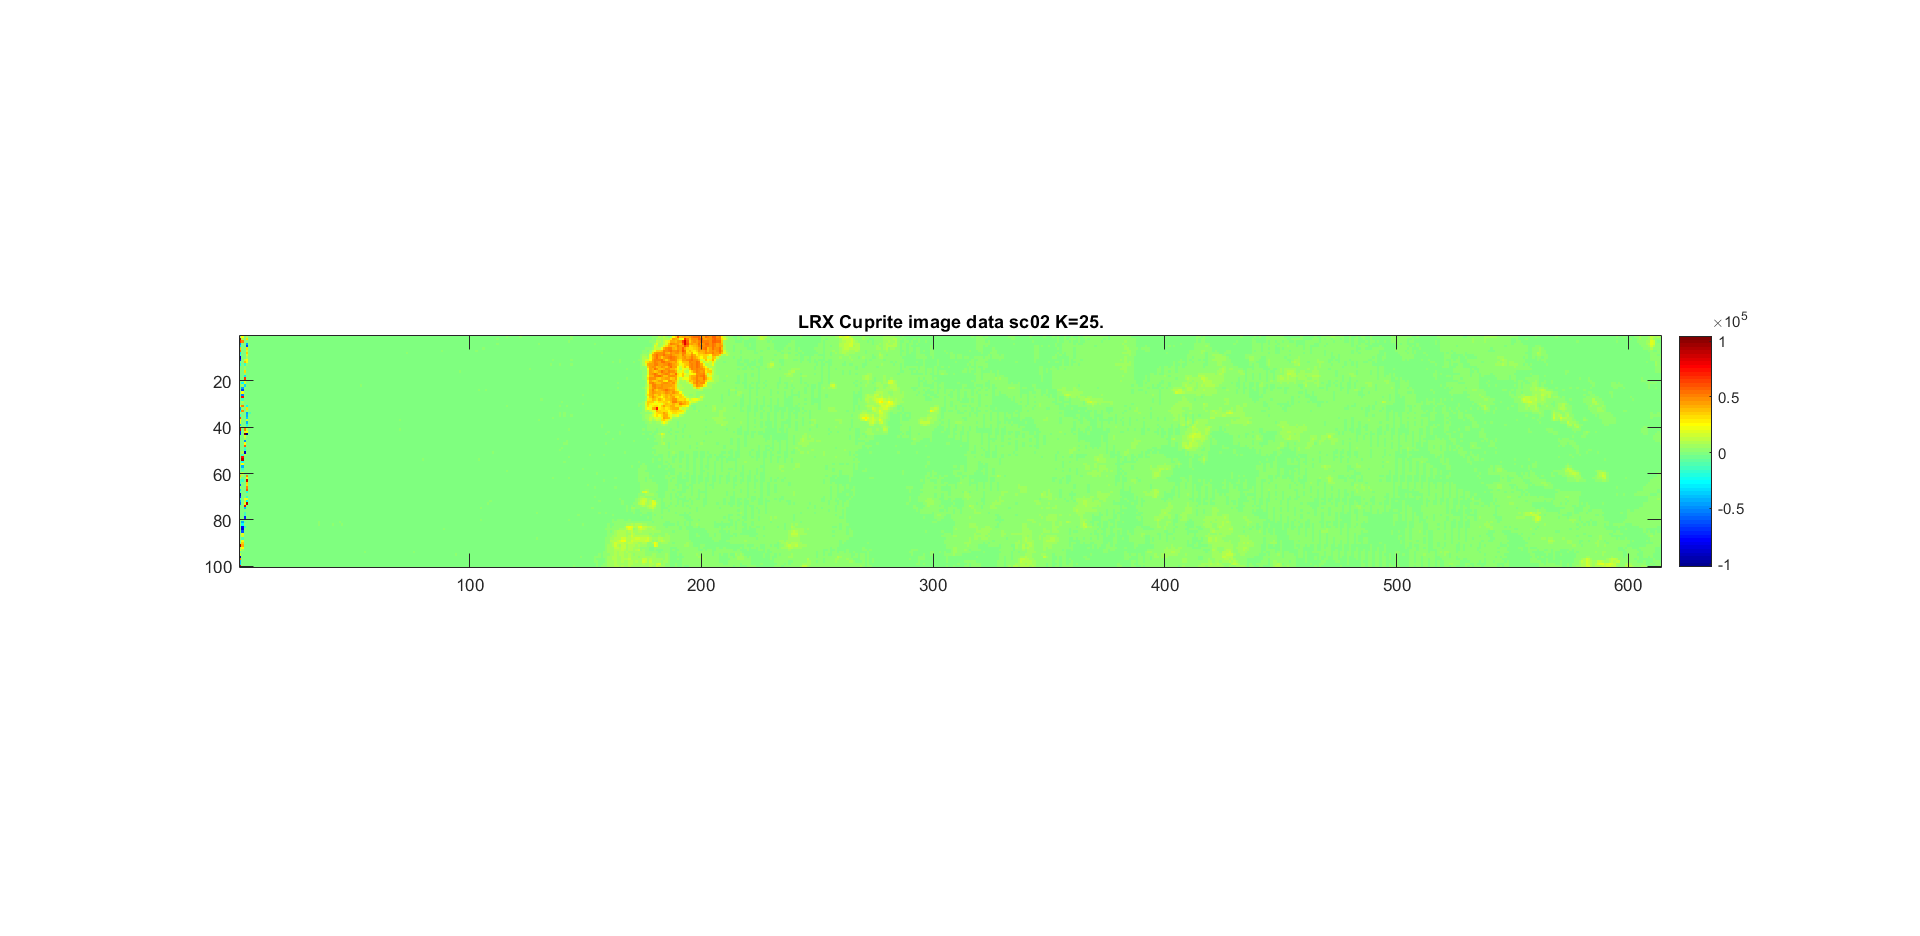
\includegraphics[scale=0.6]{images/AD_testing/hyperspectral_images/real_images/K=25_using_gauss_jordan_colormap_jet.png}}
  \caption{Result from LRX AD with a kernel size of K=25 on Cuprite image scene 02. Higher score indicates higher probability of the pixel being anomalous. } 
  \label{fig:cuprite_scene_band_220}
\end{figure}

\subsection{ALRX}

\subsection{ACAD}

ACAD is causal and computes the correlation matrix on a casual data set, back to the $N_{acad}$ previous pixel. This is further described in section \ref{sec:ACAD_theory}.

\begin{figure}[H]
\centering                                                           

   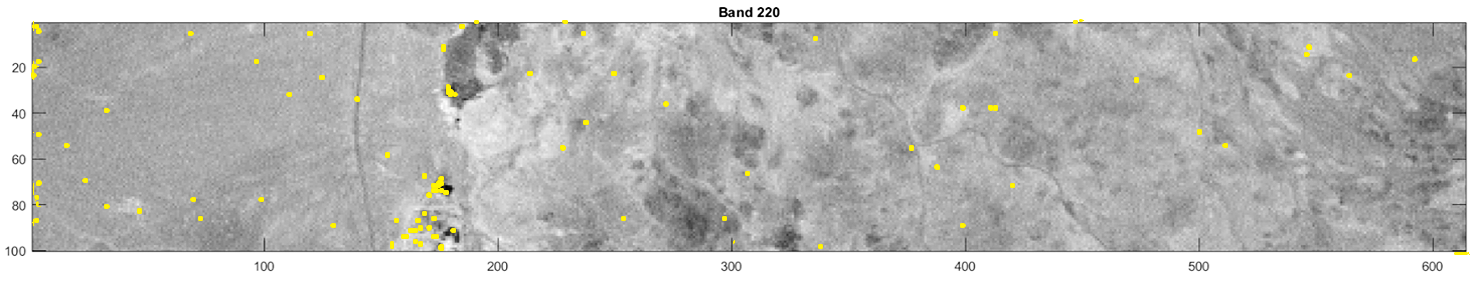
\includegraphics[scale=0.3]{images/AD_testing/anomaly_map_over_picture_tresh=250.png}
  \caption{Anomaly map created by ACAD( yellow dots) overlayed over Figure \ref{fig:cuprite_scene_band_220}. $\tau$ is set to 250.} 
  \label{fig:cuprite_scene_band_220}
\end{figure}
 
 \subsection{Choice of anomaly detector algorithm}
 
 \begin{table}[H]
\centering
 \resizebox{1.1\textwidth}{!}
{\begin{tabular}{l|l|l|l|l|l}
\textbf{AD}    & \textbf{$false\_anomalies$} &\textbf{ $\%correctly\_predicted\_$} &\textbf{Performance on} & \textbf{Possibility of}  & \textbf{Degree of}                          \\
& & \textbf{$anomalies$}& \textbf{real data}& \textbf{implementing in real time} &\textbf{parallelism}\\
\hline
RX & Hsueh :0&Hsueh: 0.3714 & Medium&Low. Need global covariance &Low.Need global covariance \\
&$Sim30\_30AVIRIS:0$ & $Sim30\_30AVIRIS$ : 1 &  & matrix before computing&matrix before computing \\
&$Sim\_Aviris01:0$ & $Sim\_Aviris01$ : 1 & & inverse. & inverse. This matrix must \\
& & & & &be computed in series.\\
LRX & & & & & \\
ALRX & & & & & \\
ACAD & & & & & \\
\end{tabular}}
\caption{Comparison of different anomaly detectors}
\label{tab:ad_comparison}

\end{table}